% !TEX root = main_min_disc_dist.tex
\subsection{Double Integrator}
The doube integrator consists of two states $(x_1, x_2)$ , and  control $u \in [u_{min}, u_{max}]$ with dynamics,
\begin{equation}
\begin{split}
\dot{x_1} & = x_2 \\
\dot{x_2} & = u 
\end{split}
\end{equation}
\noindent The state space is discretized into a $161 \times 161$ grid on the domain $[-1,5] \times [-5,5]$, and $u_{max}=-u_{min}=2$.

The task is to keep the state trajectory inside the box $\K = [0,4] \times [-3,3]$, thus the target is taken to be its compliment $\T=\K^C$. For ease of exposition we define the \emph{safe set} $\Omega(\T) := \R(\T)^C$.

We first show, in Fig~\ref{fig:convergence} that different level curves of $Z$ over approximates~(bold line) and under approximates~(dotted lines) the analytic safe set~(shown in black) for two values of $\lambda = 0.1, 0.2$, with$\bar{\tau}=2$. As expected smaller values of $\lambda$, yield tighter approximations. 

\begin{figure}
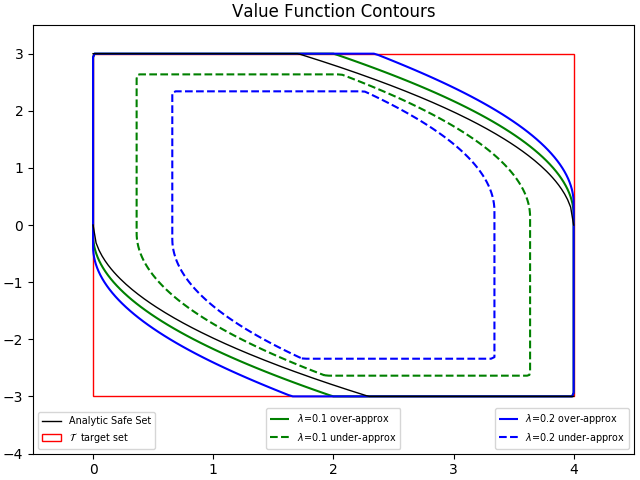
\includegraphics[scale=0.5]{convergence_difflambda.png}
\caption{The analytic safe set and target set $\mathcal{T}$ are shown in black (interior) and red (exterior), respectively. The over and under approximated $Z$ are shown in bold green and dotted green for $\lambda=0.1$; and bold blue and dotted blue line for $\lambda  = 0.2$ (all interior).}
\label{fig:convergence}
\end{figure}

We next compare value iteration and policy iteration with increasing number of discrete actions in Table~\ref{tab:v_vs_p}. In the table we see that the runtime of value iteration increases linearly with the increase in the number of actions, and policy iteration scales much better. The overall runtime favors value iteration, but it is important to note that the majority of the time in policy iteration is spent constructing $P_{\pi_u}$, which is denoted by $T_{P_{\pi_u}}$.\footnote{The data structure used to represent the interpolation is very efficient for sparse matrix multiplication, but is not ideal for indexing.}. Excluding this cost, policy iteration becomes more attractive.
\begin{table}
\centering
\caption{Value Iteration vs Policy Iteration}
\label{tab:v_vs_p}
\begin{tabular}{|c| c| c| c|}
\hline
\# actions & VI & \multicolumn{2}{|c|}{Policy Iteration} \\ \cline{3-4}
 &  $T_{total} $ & $T_{total}$ & $T_{total} - T_{P_{\pi_u}}$ \\ \hline
2 & 1.255  & 68.793  & 0.105 \\ \hline
50 &  7.562 &  69.717 & 0.365 \\ \hline
250 & 32.841 &  251.39 & 3.504 \\ \hline
500 & 63.815 &  253.855 & 6.741 \\
\hline
\end{tabular}
\end{table}

Finally, to verify the convergence properties of the MDR formulation we initialize value iteration with the zero vector $\vec{0}\in \RR^{N_G}$ with $\lambda=0.1$. The error (in the infinity norm) between the converged solution and the one visualized in Fig~\ref{fig:convergence} is $0.000299$, suggesting convergence to the same fixed point. Under the MR setting value iteration fails to converge with this particular initialization.


